En esta sección se detallan las decisiones infraestructurales tomadas para llevar la arquitectura mencionada en la sección de \nameref{sec:architecture}, 
a la práctica teniendo en cuenta el uso de recursos de las aplicaciones, el presupuesto del equipo y las necesidades actuales, 
a su vez permitiendo el escalamiento y crecimiento del proyecto.

Por otro lado, se especifica el proceso de integración y despliegue de código de forma continua y por versiones,
como también las revisiones automatizadas de errores de código, inconsistencia de formatos y de filtrado de credenciales.

\subsubsection{Proveedor de infraestructura como servicio (IaaS) elegido}

Se optó por \textit{AWS (Amazon web services)} como plataforma principal para la infraestructura (\textit{Cloud provider}) de \textbf{Feed the Realm}
debido a la flexibilidad frente a soluciones PaaS, alcance global, madurez del ecosistema y familiaridad por parte del equipo con sus herramientas.
Durante la elección del proveedor también se consideraron alternativas como Linode, Hetzner, 
GCP \textit{(Google cloud platform)} y Microsoft Azure.

Uno de los factores más relevantes fue la capacidad de construir una infraestructura altamente modular y flexible.
En lugar de depender de un entorno excesivamente administrado o centrado únicamente en plataformas PaaS,
se priorizó mantener control directo sobre la orquestación, el networking y el ciclo de despliegue de servicios.

Otro punto importante fue la capa de almacenamiento y distribución de contenido, ya que el juego debía permitir
a los creadores subir un volumen importante de modelos 3D y cosméticos 2D, y a los jugadores descargar los mismos sin
altos tiempos de descarga. Para esto se eligió combinar el servicio de Amazon S3 junto con CloudFront como 
\textit{CDN (content delivery network)} por la sencilla integración que ofrece.

En comparación con Linode y Hetzner, AWS ofrecía un ecosistema considerablemente más completo en términos de automatización,
segmentación de infraestructura, seguridad y herramientas operativas. Aunque proveedores como Hetzner destacan por sus bajos precios
no cuentan con componentes críticos como políticas IAM \textit{(identity access management)}, registros de contenedores, entre otros,
lo que significaría un mayor esfuerzo operativo.

La decisión también estuvo influenciada por criterios de escalabilidad a largo plazo, ya que si bien el proyecto no
requiere inicialmente una infraestructura masiva, se buscó una plataforma que permitiera crecer progresivamente 
sin necesidad de rediseñar componentes fundamentales.

\subsubsection{CI/CD \& Workflows}
\label{sec:ci-cd}

El sistema cuenta con pipelines de integración y despliegue continuo (\textit{CI/CD}) implementados mediante 
GitHub Actions, que automatizan el proceso de validación, construcción y despliegue de los distintos 
componentes del sistema. Dado que el proyecto involucra tecnologías heterogéneas, cada componente cuenta con 
su propio flujo de trabajo adaptado a sus particularidades técnicas.

\paragraph{Core-service}

En el caso del backend web 'core-service' se tiene un flujo de trabajo que inicia cuando se efectiviza una acción de \textit{Merge}
de código desde la rama de desarrollo (\textit{dev}) hacia la rama de despliegue (\textit{main}).

Como se puede apreciar en la figura a continuación se comienza por la ejecución de las pruebas, luego si estas son exitosas se pasa
al siguiente paso donde se construye la imagen de docker del servicio y finalmente si esta etapa también se completa con éxito
se lleva a cabo el despliegue en \textit{AWS EC2}.

\begin{figure}[H]
\centering
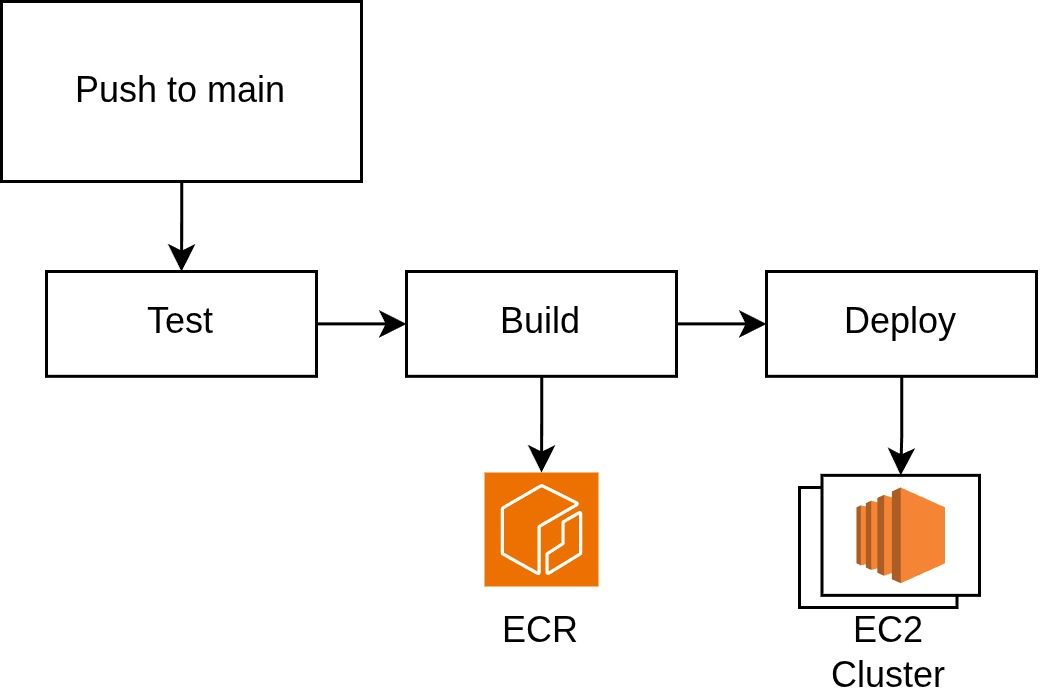
\includegraphics[width=0.5\textwidth]{img/09-technical-details/devops/core-workflow.jpg}
\caption{Visión general del 'workflow' de integración y despliegue continuo del \textit{core-service}.}
\end{figure}

En la etapa de pruebas se lleva a cabo la ejecución de un \textbf{docker-compose} y de tests de aceptacion haciendo
uso de la libreria de python \textbf{'Behave'} para \textbf{'Gherkin'} con el objetivo de validar el comportamiento
del servicio de manera externa, y tambien se ejecutan tests unitarios con el objetivo de asegurar el correcto funcionamiento
de cada una de las partes individualmente.

Luego se calcula el cubrimiento o \textit{'coverage'} del codigo utilizando la herramienta \textbf{CodeCov}
y de esta forma obtener un porcentaje descriptivo de la confiabilidad del codigo (frente a lo esperado),
asi como tambien visualizar las partes del codigo con menor cubrimiento por medio de gráficos varios.

\begin{figure}[H]
\centering
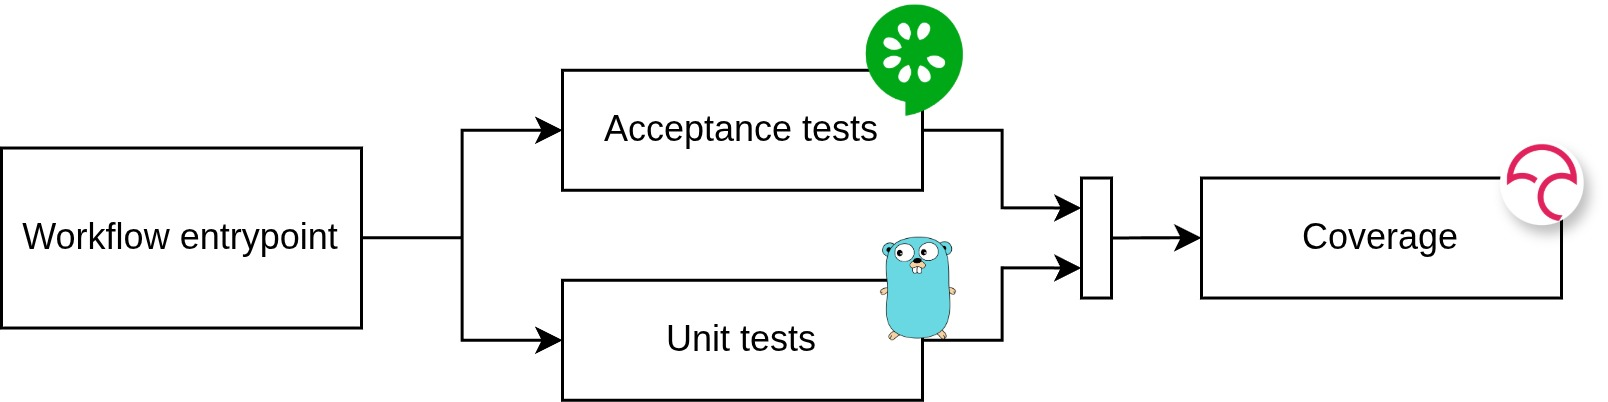
\includegraphics[width=0.75\textwidth]{img/09-technical-details/devops/test-pipeline.jpg}
\caption{Pipeline de ejecución de Tests.}
\end{figure}

En la etapa de construcción (una vez concluyó exitosamente la etapa de testing) se realizan dos tareas bloqueantes antes
de subir la imagen al registro de contenedores, estas son las siguientes:

\begin{itemize}
    \item \textbf{Build}: Se realiza la construcción per-se de la imagen utilizando docker y el \textit{Dockerfile}
        con el objectivo o \textit{'target'} correspondiente.
    \item \textbf{Elastic Container Registry Login}: Se realiza la obtencion de un token \textit{OIDC (OpenID connect)} utilizando 
        a \textit{Github} como proveedor, para de esta forma poder utilizar \textit{AWS STS (security token service)}
        y verificar la identidad del pipeline obteniendo asi acceso al corresponiente rol de 
        \textit{IAM (identity access management)} que permite realizar la operacion de subida de la imagen al registro
        de contenedores de AWS, \textbf{ECR}.
\end{itemize}

\begin{figure}[H]
\centering
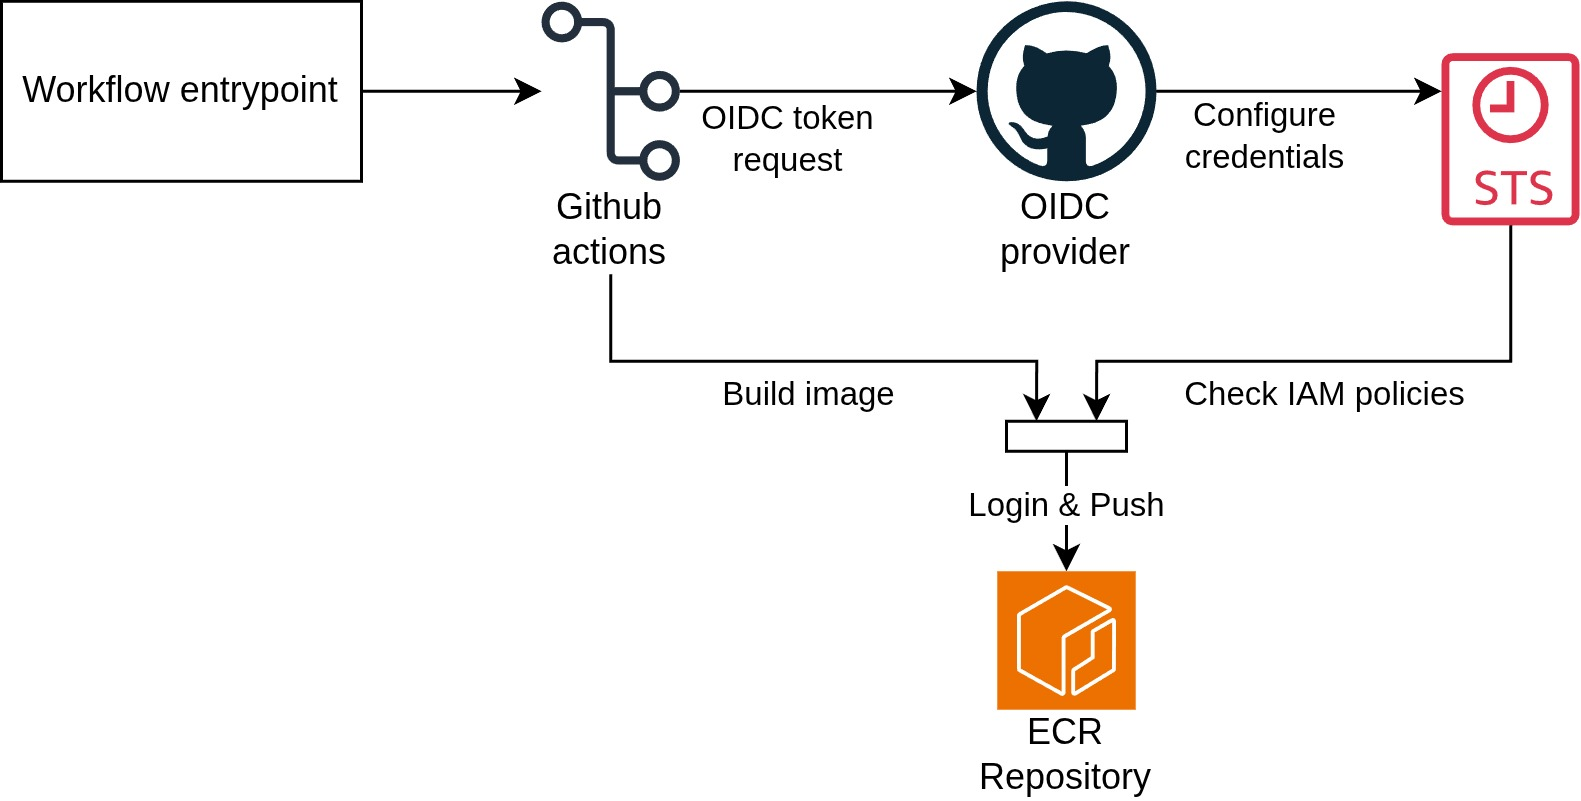
\includegraphics[width=0.75\textwidth]{img/09-technical-details/devops/build-pipeline.jpg}
\caption{Pipeline de construcción de la imagen de docker y subida a ECR.}
\end{figure}

Finalmente, se llega a la etapa de despliegue (una vez conluida la anterior sin errores).
En esta etapa se lleva a cabo la misma configuración para tener acceso al rol IAM que permite también enviar comandos
\textit{SSM (systems manager)} cuyo propósito es comunicarse de manera segura con una de las instancias de \textbf{EC2} objetivo,
sin exponer puertos para comunicación por \textit{SSH}, y de esta manera ejecutar un script que consiste en la obtención de la imagen
desde \textbf{ECR} y la ejecución el contenedor por medio de \textit{docker run}.

\begin{figure}[H]
\centering
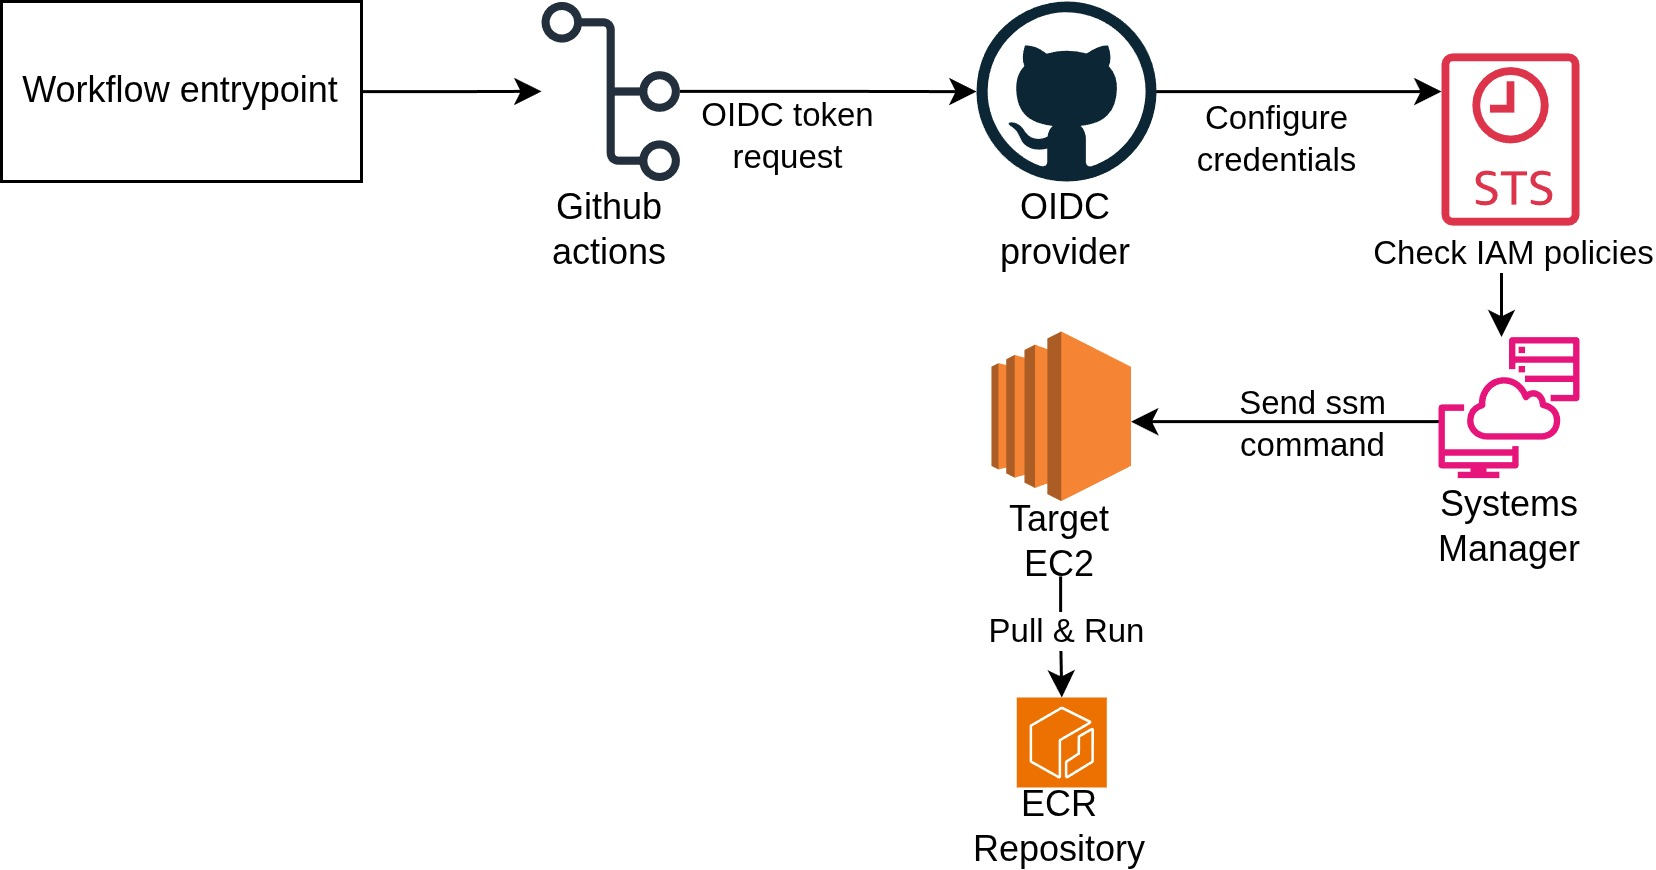
\includegraphics[width=0.8\textwidth]{img/09-technical-details/devops/deploy-pipeline.jpg}
\caption{Pipeline de despliegue del contenedor y ejecución en EC2.}
\end{figure}

\paragraph{Zoning servers o ftr-servers}

Por otro lado, en el caso de los \textir{zoning servers} o \textit{ftr-servers} se tiene un flujo de trabajo que inicia cuando 
se crea y se sube al repositorio una nueva etiqueta o \texit{tag} de versión con el formato de versionamiento semántico \textbf{vX.Y.Z}.

Sin embargo, al tratarse de una aplicación confeccionada en \textif{Unity}, esta debe ser compilada utilizando el correspondiente compilador
propietario y haciendo uso de una licencia que lo permita.
Esto impone una serie de trabas al momento de realizar un pipeline de integración y despliegue continuo, no solo por la inexistencia
de herramientas oficiales para la compilación en un entorno de \textit{'Github actions'} siendo la única herramienta oficial para
este propósito, una externa al control de versiones utilizado, lo que forzaría al equipo a mantener dos controles de 
versiones (git y \textit{Unity versión control}), sino también por la necesidad de obtener y descargar paquetes de dependencias
(cada uno con su licencia) desde dentro del entorno de compilación.

Es por esto que se optó por la compilación local de los ejecutables y su contenerización incluyendo el ejecutable optimizado
para servidores \textit{Linux} en la imagen de docker, para ser subida a \textit{GHCR (Github container registry)}.

Una vez que dicha imagen se encuentra alojada en el registro de contenedores, se realiza el etiquetado del \textit{commit} a desplegar
y se ejecuta automaticamente el \textit{pipeline} que como se ve en la siguiente figura, obtiene la imagen de dicho alojamiento y (haciendo el mismo procedimiento del core-service explicado anteriormente)
la sube a \textbf{ECR}, para finalmente notificar por medio de un \textbf{webhook} al core-service que se deben actualizar todos
los zoning servers (ftr-server) que se encuentran activos en ese momento.

\begin{figure}[H]
\centering
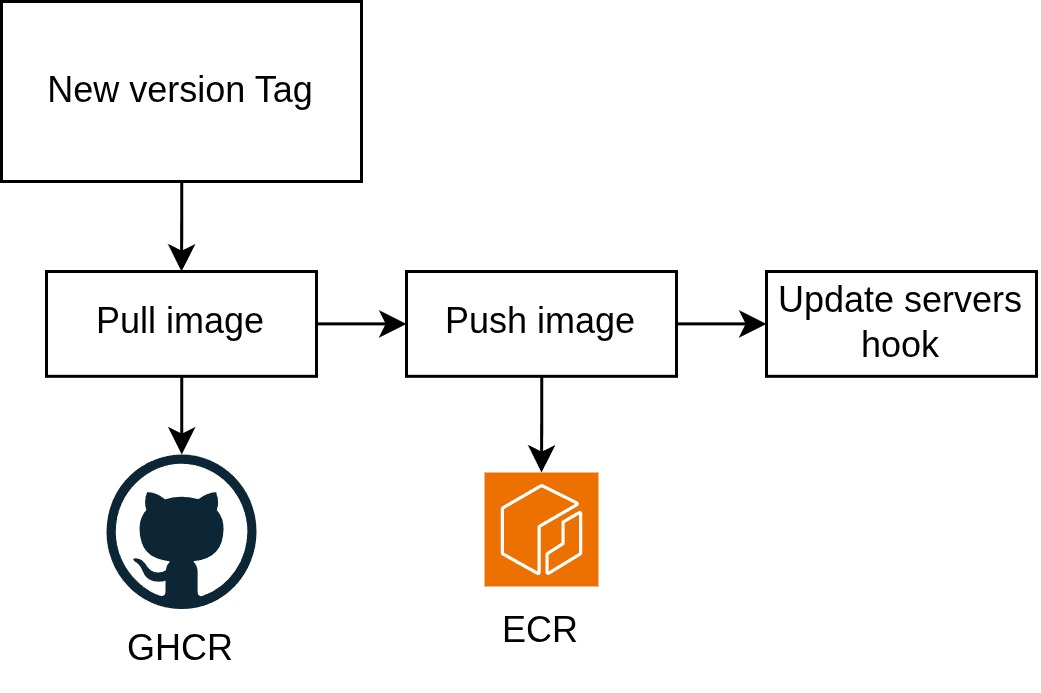
\includegraphics[width=0.5\textwidth]{img/09-technical-details/devops/server-workflow.jpg}
\caption{Visión general del 'workflow' de actualización de la imagen de los \textit{ftr-server}.}
\end{figure}

\subsubsection{Actualización de las aplicaciones 'Cliente'}

En el caso de las aplicaciones cliente, es decir, el editor de mundos y el juego, al igual que con la imagen 
de docker de los servidores (\textit{ftr-server}), estas no se compilan en un pipeline de integración continua 
debido a las limitaciones impuestas por Unity, sino que son compiladas manualmente por un miembro del equipo. 
Por el momento solo se compilan para las plataformas de Windows y Linux.

\vspace{0.25cm}

Luego de ser compiladas, se comprimen y se realiza un \textit{Release} de la nueva versión a través del sistema \textit{Back Office} que se abordara en la correspondiente sección.
De esta forma los usuarios tendrán acceso a la última versión disponible de las aplicaciones obteniéndolas de la página principal del juego.

\subsubsection{Infraestructura}
\label{sec:infrastructure}

A continuación se explica el estado actual de la infraestructura cuya especificación y configuración pertenece al repositorio
de \textbf{IaC}, el cual define la misma por medio de la herramienta \textbf{Terraform}, como también la solución implementada para el despliegue
\textit{on-demand} de mundos y zoning servers, y para el \textit{discovery} de servicios de forma dinámica que tiene
como objetivo que los jugadores puedan establecer una conexión directa con el servidor en el que desean jugar.

\paragraph{Elección del orquestador de servicios}

La elección de \textbf{HashiCorp Nomad} como orquestador de cargas de trabajo respondió tanto a criterios operativos como económicos.

Si bien \textbf{Kubernetes} constituye actualmente el estándar de facto para la orquestación de contenedores, muchas de sus capacidades están orientadas a entornos
de gran escala y alta complejidad operativa, en el caso de \textbf{Feed the Realm}, donde los servidores de juego representan sesiones activas con jugadores conectados
en tiempo real, se priorizó un modelo de \textit{scheduling} más predecible y controlado.
Kubernetes puede realizar procesos automáticos de re-balanceo, reprogramación o reemplazo de \textit{pods} cuando detecta cambios en la disponibilidad de recursos del clúster, y
si bien este comportamiento resulta beneficioso para aplicaciones web sin estado (\textit{stateless}), puede provocar la finalización y recreación 
de una instancia de servidor de juego durante una partida, desconectando a todos los jugadores conectados a la misma.
Nomad, por el contrario, adopta una filosofía más simple y conservadora respecto de la reasignación de cargas, permitiendo mantener los procesos ejecutándose 
en el nodo asignado hasta que exista una razón explícita para migrarlos o reiniciarlos.

Asimismo, desde la perspectiva de costos, Nomad presenta una ventaja significativa al requerir una cantidad considerablemente menor de componentes de control para operar.
Un clúster básico puede ejecutarse con pocos servicios y un consumo reducido de memoria y CPU, mientras que Kubernetes suele requerir una mayor cantidad de procesos 
auxiliares y, en entornos administrados como \textit{EKS (Elastic Kubernetes Service)}, implica además costos asociados al plano de control independientemente 
de la carga real del sistema.

Dado que la infraestructura de \textit{Feed the Realm} busca desplegar servidores bajo demanda y optimizar el uso de recursos disponibles,
se consideró que Nomad ofrecía una mejor relación entre simplicidad operativa, previsibilidad del comportamiento y costo de mantenimiento, sin sacrificar las capacidades 
necesarias para el crecimiento futuro del proyecto. En conjunto con Nomad se utilizara \textbf{HashiCorp Consul} que provee
herramientas para monitoreo de contenedores por medio de \textit{healthchecks} y descubrimiento de servicios (\textit{Service Discovery}).

\paragraph{Componentes principales}

Las partes principales de la infraestructura son:
\begin{itemize}
    \item \textbf{Nomad server node - EC2}: Este tipo de nodos son los que contienen mínimamente
        una instancia de \textit{nomad server} y otra de \textit{consul server}.
    \item \textbf{Nomad client node - EC2}: Este tipo de nodos contienen mínimamente una instancia
        \textit{nomad client} y otra de \textit{consul client}. A su vez son los que se utilizaran para desplegar los ftr-servers.
    \item \textbf{Buckets - S3}: Utilizados para almacenamiento de archivos de imágenes para cosméticos o ítems,
        y archivos de modelos 3D asignados a cada mundo.
    \item \textbf{CDN - CloudFront}: Red de distribución de contenido utilizada para él cache geográficamente cercano a los clientes
        de los archivos descargados de manera de disminuir los tiempos de descarga futuros.
    \item \textbf{Registro de contenedores  - ECR}: Utilizado para almacenar las imágenes de docker de cada versión lanzada
        de cada servidor desplegable, y para el escaneo general automatizado de vulnerabilidades en las mismas.
    \item \textbf{PostgresDB - Supabase}: Base de datos PostgresSQL alojada en \textit{Supabase} a ser utilizada por el core-service.
    \item \textbf{MongoDB - Mongo Atlas}: Base de datos Mongo utilizada por los 'zoning servers' para persistir información de los jugadores
        en los mundos. Se crea una base de datos por mundo dentro del mismo \textit{cluster}.
    \item \textbf{Firewall - Security Groups}: Whitelist de puertos que permiten tráfico entrante o saliente para cada tipo de nodo.
    \item \textbf{Permisos \& Roles - IAM}: Configuración de roles para cada tipo de nodo o usuario y permisos específicos
        y mínimos para los mismos.
    \item \textbf{Monitoreo - Datadog}: \textit{Deamonset} o \textit{Agente} de Datadog para recolección de métricas de uso de recursos,
        lanzados al inicio de cada nodo.
    \item \textbf{DNS - Route53}: Configuración de registros DNS para el dominio (apex) y los subdominios utilizados.
    \item \textbf{Páginas web - Vercel}: Despliegue de \textit{backoffice} y \textit{landing page} en Vercel, a través de \texit{pipelines}
        ejecutados cuando se realiza un \textit{push} a la rama principal de cada repositorio.
\end{itemize}

En la siguiente figura se puede apreciar algunos de los componentes mencionados, como están separados a nivel físico, qué servicios alojan y como se conectan entre sí.

También se puede notar la intercomunicación de los nodos de tipo 'nomad client', esto es crucial para el funcionamiento del descubrimiento de
servicios por nombre. Tanto esto como el flujo de despliegue de nuevos 'zoning servers' se aborda en detalle a continuación.

\begin{figure}[H]
\centering
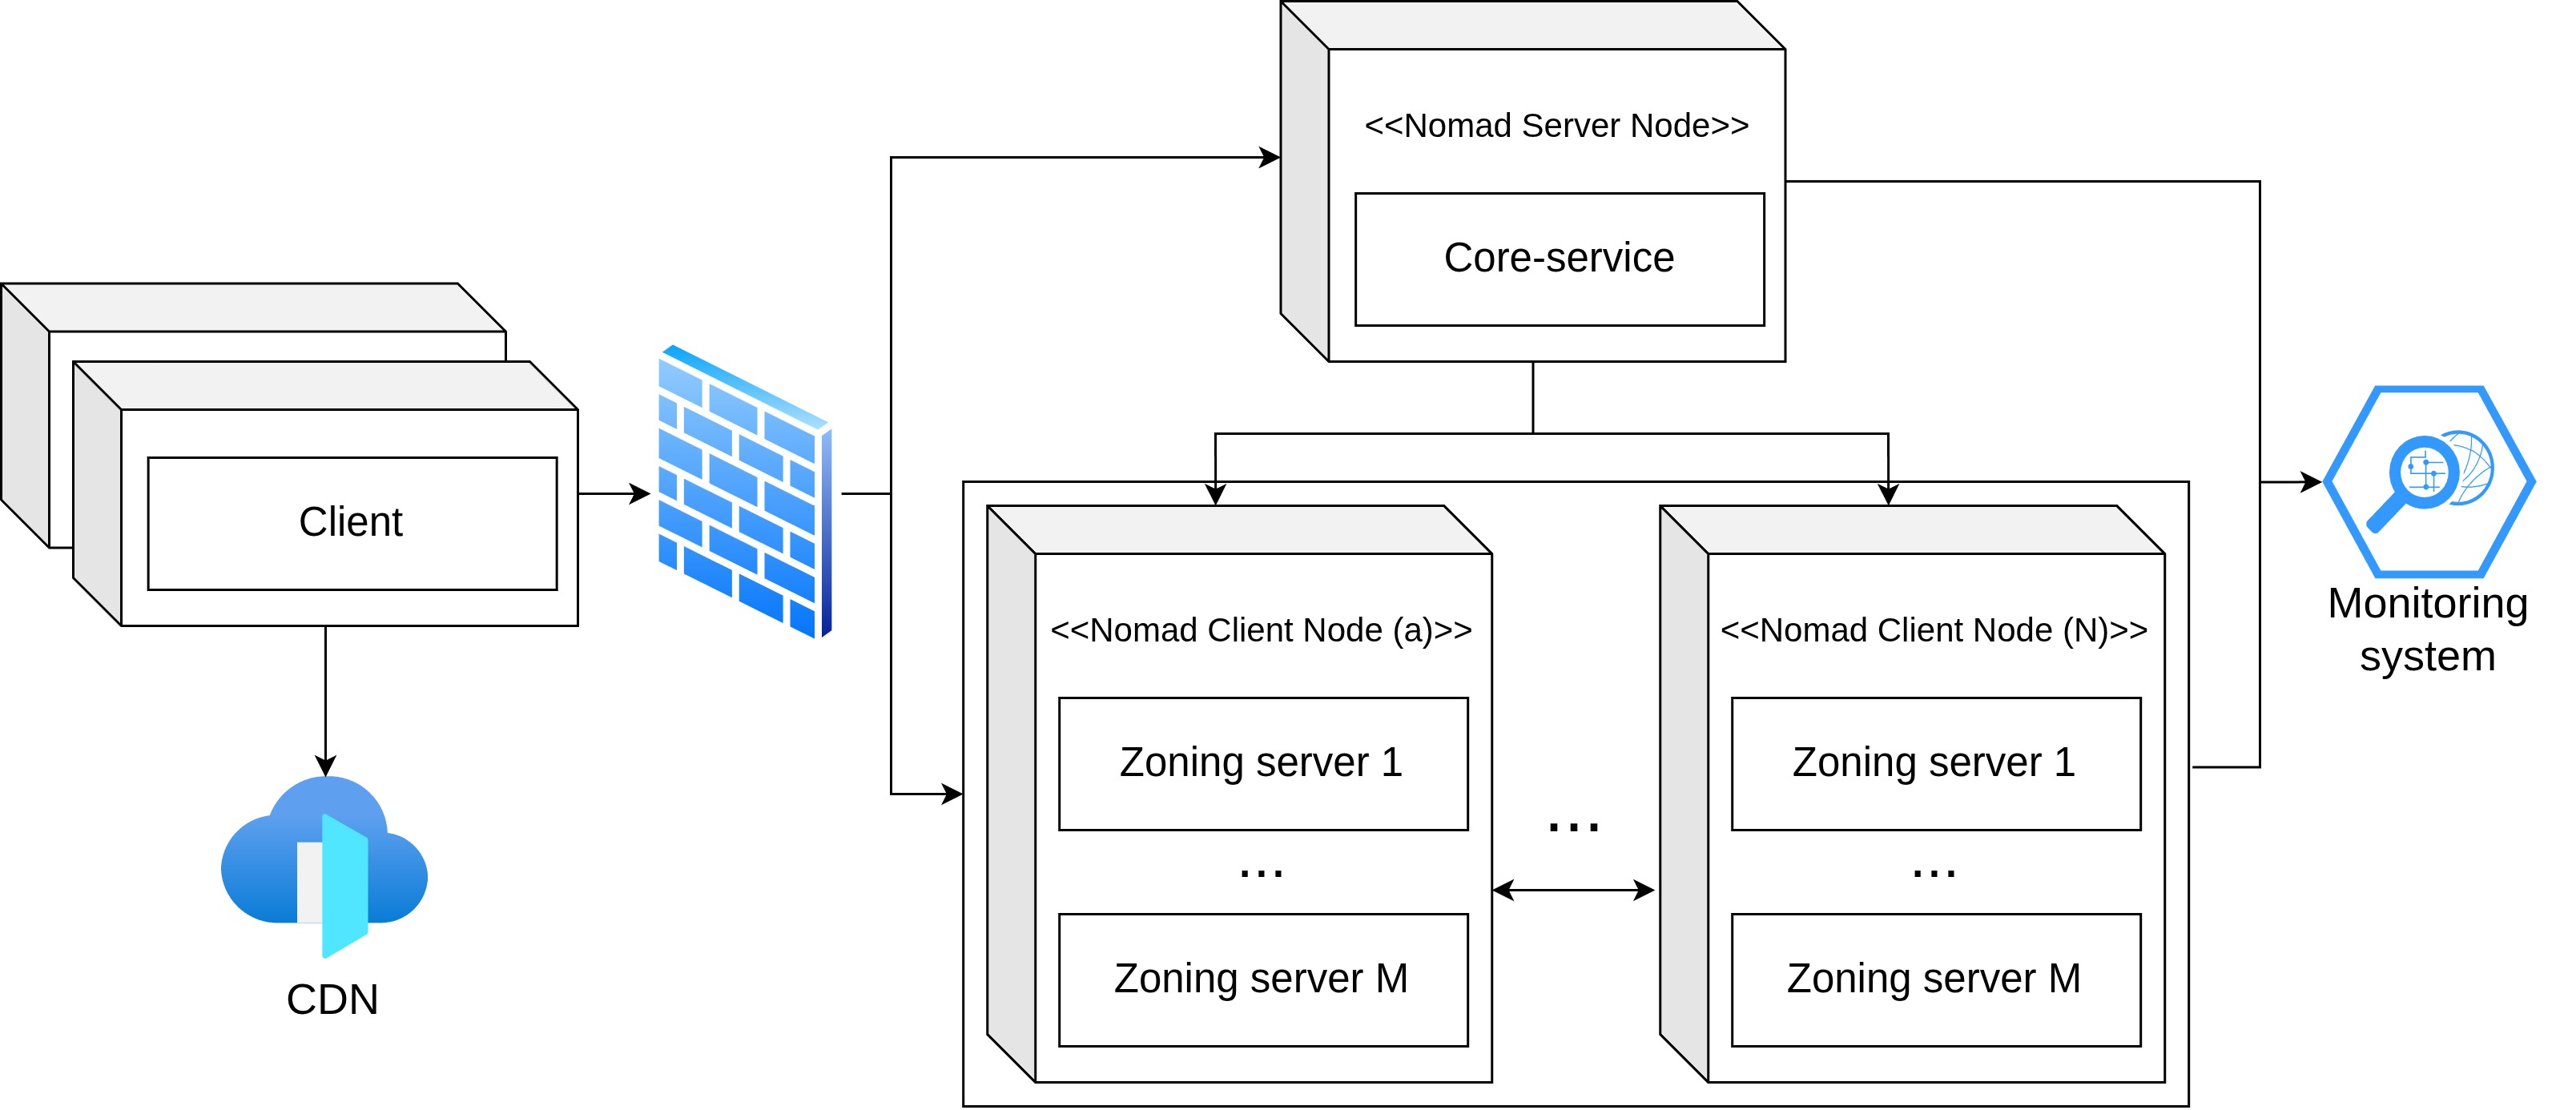
\includegraphics[width=1\textwidth]{img/09-technical-details/devops/deployment.jpg}
\caption{Vista general de la infraestructura desplegada.}
\end{figure}

\paragraph{Orquestación, Descubrimiento y Comunicación de Servicios}

Los clientes interactuan con los servicios desplegados de dos formas principales:
\begin{enumerate}
    \item A través de un \textit{API Gateway} (\textit{Nginx} en este caso) que se encarga de gestionar las conexiones seguras mediante TLS
        utilizando certificados administrados y renovados por \textit{Certbot}, de validar el tamaño de los archivos enviados,
        y de enrutar los requests al core-service.
    \item Por socket para una comunicación directa con los servidores del juego con el objetivo de disminuir la latencia/\textit{overhead}
        de un 'gateway' o balanceador de carga.
\end{enumerate}

En cuanto al servicio backend web \textbf{core-service}, este recibe peticiones de parte de los usuarios ya sea tanto jugadores como administradores,
y utiliza para resolver las mismas una serie de dependencias como lo son:
\begin{itemize}
    \item Base de datos PostgresSQL alojada en Supabase y contra la cual se ejecutan las consultas relacionales.
    \item Buckets de \textbf{'cosmetics'} y \textbf{'content'} para almacenamiento de imágenes png y modelos 3D cuyas URIs
        son guardadas en la base de datos por el core-service. A su vez utiliza archivos temporales para evitar mantener en memoria
        los archivos siendo subidos en su totalidad.
\end{itemize}

\begin{figure}[H]
\centering
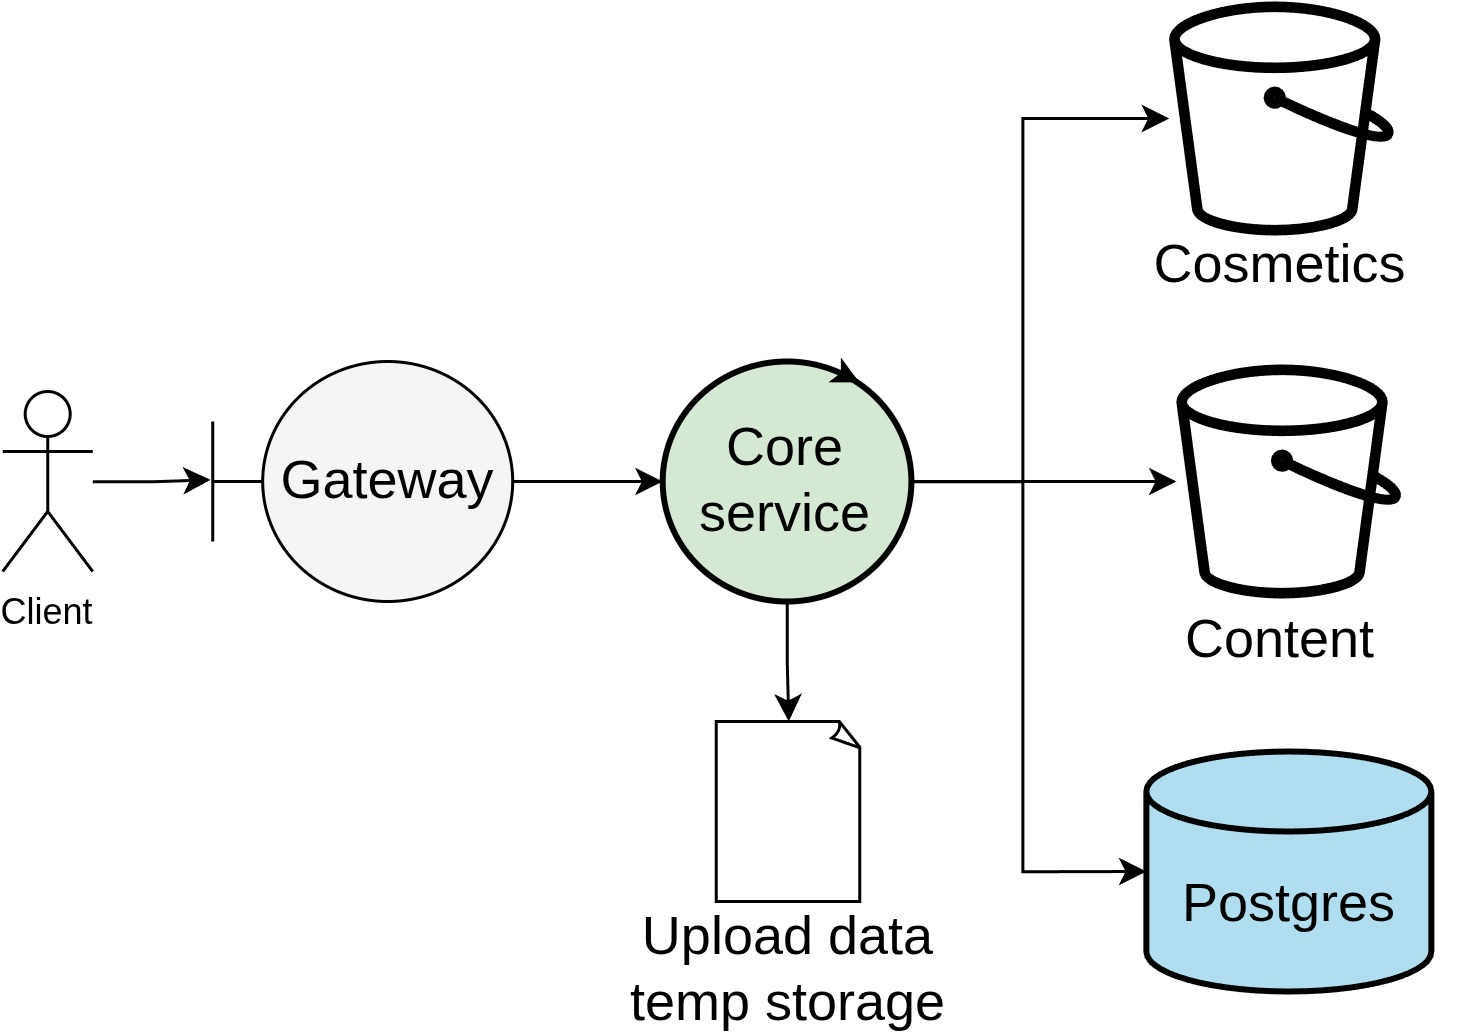
\includegraphics[width=0.5\textwidth]{img/09-technical-details/devops/core-robust.jpg}
\caption{Diagrama del uso del core-service y sus dependencias.}
\end{figure}

Por otro lado, el despliegue de nuevos 'zoning servers' inicia cuando un cliente de tipo 'creador' activa una o varias zonas pertenecientes a un mundo
a través del core-service.
Cuando core-service recibe esta request (luego de hacer las validaciones corresponientes), genera una especificación de \textit{Nomad Job} a partir de un
template detallado preliminarmente, para luego comunicarse de forma interna con el servicio de \textbf{Nomad server} el cual se encuentra ejecutandose 
en el mismo nodo (aunque no necesariamente) y enviarle dicha especificación.
Una vez el Nomad server obtiene el \textit{Job}, este consulta su registro de nodos cliente (quienes envian heartbeats periodicamente para notificar su estado al server)
y decide por medio de un proceso de \textit{scheduling} el nodo que debe alojar el nuevo servidor.
El nodo cliente seleccionado, entonces obtiene la imagen de docker desde el registro de contenedores y lo ejecuta con los parametros necesarios
como el \textit{ID} del mundo y de la zona activada.

Este proceso se podria hacer mas tolerante a fallos agregando nuevos \textit{Nomad servers}, ya que en el caso donde hay más de estos,
se utiliza el algoritmo \textit{RAFT} para mantener un consenso de los \textit{schedules} y las asignaciones.

\begin{figure}[H]
\centering

\includegraphics[width=0.6\textwidth]{img/09-technical-details/devops/nomad-robust.jpg}
\caption{Flujo de despliegue e inicio de zone server.}
\end{figure}

Para llevar a cabo el descubrimiento de las direcciones de los 'zoning servers' una vez ya estan desplegados se utiliza la herramienta \textbf{Consul}.

La misma requiere de la existencia de al menos un \textit{Consul server} (desplegado en el mismo nodo donde está el Nomad server) y de \textit{Consul clients}.
Los Consul clients utilizan un algoritmo de comunicación por \textit{Gossip} o 'Chisme', seleccionando aleatoriamente nodos de Consul a los que les enviara
la información del estado y la dirección (IP y puerto) de los servicios que conoce por nombre, y de esta forma la información se propaga exponencialmente en la red interna 
de Consul y llegan a su vez a los Consul servers, quienes mantienen un registro de los cambios de estado de los servicios desplegados.

Esta es la razon porque en la primera figura de esta sección se mencionó la intercomunicación de nodos de tipo \textit{'Nomad client node (N)'}, y de
esta forma se logra tener una fuente confiable de \textit{Service Discovery} para poder resolver las peticiones de los usuarios por direcciones
de los zoning servers utilizando el \textit{ID} del mundo y la zona como nombre de servicio.

Similarmente con los \textit{Nomad servers}, se podria mejorar la tolerancia a fallos del sistema de descubrimiento agregando nuevos \textit{Consul servers},
ya que los mismos también usan el algoritmo \textit{RAFT} para mantener consenso entre ellos.

\begin{figure}[H]
\centering

\includegraphics[width=0.6\textwidth]{img/09-technical-details/devops/consul-robust.jpg}
\caption{Flujo de descubrimiento de dirección de zone server (por mundo y zona).}
\end{figure}

Finalmente, una vez que el jugador ya obtiene la dirección del servidor en el que desea jugar, este se comunica con el mismo
a través de la capa de red del juego (Utilizando UDP como base).
A partir de ese momento el jugador envía sus comandos y el servidor le responde con estados de juego o eventos (tal como se menciona en la sección de \textit{Netwoking} del juego),
a su vez el zoning server almacena la información del jugador en la base de datos Mongo perteneciente al mundo y alojada en \textit{Mongo Atlas}.

\begin{figure}[H]
\centering

\includegraphics[width=0.65\textwidth]{img/09-technical-details/devops/game-robust.jpg}
\caption{Diagrama de uso de zone server y sus dependencias \textit{(cliente in-game)}.}
\end{figure}

\paragraph{Configuración de DNS}

La resolución de nombres del sistema se implementó mediante \textit{Amazon Route 53}, definiendo tanto una zona pública para el dominio \textbf{feedtherealm.world}
como una zona privada interna utilizada exclusivamente por los servicios desplegados dentro de la VPC (\textit{virtual private cloud}).

En la zona pública se configuraron registros que permiten acceder a los distintos componentes de la plataforma,
incluyendo el dominio raíz (apex), los subdominios \textbf{www}, \textbf{admin} y \textbf{core}, además de un conjunto dinámico de registros 
(\textbf{s1}, \textbf{s2}, \dots) asociados a las direcciones IP públicas de los nodos clientes de Nomad que pueden alojar servidores de juego.
Asimismo, se añadieron los registros TXT y CNAME requeridos para la autenticación y validación del servicio de correo electrónico utilizado por 
la plataforma, los cuales se envian desde \textbf{'noreply@feedtherealm.world'}.

Por otro lado, la zona privada \textbf{internal} proporciona un mecanismo de resolución de nombres para la comunicación entre servicios dentro de la infraestructura.
En ella se registran direcciones internas para componentes como \textbf{nomad.internal}, \textbf{consul.internal} y \textbf{core-service.internal},
evitando la dependencia de direcciones IP estáticas y simplificando la configuración de los servicios.
Esta separación entre DNS público e interno permite exponer únicamente los componentes necesarios hacia Internet mientras que la comunicación entre servicios permanece 
aislada dentro de la red privada.

\subsubsection{Seguridad informática}

Es importante para una aplicación productiva que se tenga presente la importancia de la seguridad informática,
y que se tomen medidas para proteger los sistemas, datos y usuarios frente a posibles amenazas o ataques.

Los cuidados que se tuvieron en cuenta para el desarrollo de los sistemas asociados a \textit{Feed the Realm} son:

\begin{itemize}
    \item \textbf{TLS}: Encriptado de las comunicaciones con el servicio web para garantizar la seguridad
        de los datos en tránsito.
    \item \textbf{Privilegios mínimos}: Se apunta a crear roles con permisos específicos para cada necesidad,
        siendo seguro (sin permisos) por defecto. También se mantiene un usuario administrador de AWS (utilizado para operaciones de despliegue) separado del usuario
        \textit{root} (el cual tiene el método de pago).
    \item \textbf{Firewall}: Como se mencionó anteriormente, se tiene una definición a modo de \textit{Whitelist} de los puertos que se exponen al público para cada nodo,
        definiendo solamente los puertos necesarios. Se evita exponer puertos utilizados por servicios como \textit{Nomad} o \textit{Consul}.
    \item \textbf{Reporte de bugs}: Además de los errores que pueden ocurrir y detectarse a nivel del juego, también se reportan en \textit{github issues}
        errores de código y lógica detectados que llevan a posibles \textit{exploits} o \textit{cheats}.
    \item \textbf{Almacenamiento de credenciales}: Las variables no secretas se guardan en texto plano en el repositorio de \textit{IaC}, mientras que
        las que requieren un manejo cauteloso por ser críticas para las comunicaciones con servicios externos o para firmas internas se suben a través de
        terraform como \textit{SecureString} a \textit{AWS SSM Parameter Storage}, desde donde se toman para inyectar a los contenedores como variables de entorno.
        También, como parte de los \textit{Pipelines} ejecutados en cada push a cada repositorio y los \textit{Precommit hooks} se analiza el posible filtrado de credenciales con \textbf{gitleaks}.
    \item \textbf{Escaneo de vulnerabilidades}: Se realizan controles automáticos para detectar vulnerabilidades tanto en las imágenes de contenedores 
        como en las dependencias (paquetes)  utilizadas por los proyectos. 
        Las imágenes de Docker se analizan al ser publicadas en el registro de contenedores, mientras que las dependencias son verificadas mediante \textbf{OSV-Scanner},
        identificando paquetes afectados, la severidad de las vulnerabilidades y el detalle de los \textit{CVE} reportados.
    \item \textbf{Terraform state}: Se guarda el estado de terraform luego de aplicar cambios en un bucket asegurado con bloqueo de acceso público y cifrado de los datos
        en tránsito y en reposo.
\end{itemize}
